\documentclass[11pt,a4paper]{article}
\usepackage{fontspec}
\usepackage{polyglossia}
\setdefaultlanguage{russian}
\setotherlanguage{english}
\defaultfontfeatures{Ligatures=TeX}
\setmainfont[
  Path=fonts/,
  UprightFont=cmunrm.otf,
  BoldFont=cmunbx.otf,
  ItalicFont=cmunti.otf,
  BoldItalicFont=cmunbi.otf,
  Ligatures=TeX
]{CMU Serif}
\setmonofont[Path=fonts/,UprightFont=cmuntt.otf]{CMU Typewriter Text}
\usepackage[left=2cm,right=2cm,top=2cm,bottom=3cm]{geometry}
\usepackage{amsmath,amssymb,booktabs,graphicx,float,caption,setspace,fancyvrb}
\usepackage[unicode,hidelinks]{hyperref}
\graphicspath{{figures/}}
\setlength{\parindent}{0cm}
\setlength{\parskip}{0.2\baselineskip}
\setlength{\emergencystretch}{3em}
\renewcommand{\arraystretch}{1.08}
\captionsetup{font=small}
\begin{document}
\hypersetup{pageanchor=false}
\begin{titlepage}
\centering
Федеральное государственное автономное\\
образовательное учреждение высшего образования\\
\textbf{«Национальный исследовательский университет ИТМО»}
\vfill
{\Large\bfseries Отчёт по учебно-исследовательской работе № 1\par}
\vspace{0.5\baselineskip}
по дисциплине «Моделирование»\\
\vspace{0.5\baselineskip}
\textbf{«Обработка результатов измерений:\\статистический анализ числовой последовательности»}\\
\vspace{0.5\baselineskip}
Вариант 263
\vfill
\begin{flushright}
Выполнил:\\
Чэнь Хаолинь P3316\\[1\baselineskip]
Проверил:\\
Тропченко Андрей Александрович
\end{flushright}
\vfill
\begin{center}г. Санкт-Петербург, 2026\end{center}
\end{titlepage}
\hypersetup{pageanchor=true}
\setstretch{0.95}
\tableofcontents
\newpage
\setstretch{1}

\section{Постановка задачи}
Цель работы --- исследовать числовую последовательность методами математической статистики, определить её корреляционные свойства и подобрать аппроксимирующий закон распределения по двум моментам.

Требуется обработать первые 10, 20, 50, 100, 200 и 300 значений. Для каждого объёма выборки следует найти оценки математического ожидания, дисперсии, среднеквадратического отклонения, коэффициента вариации и доверительные интервалы для среднего при вероятностях 0.90, 0.95 и 0.99. Полученные характеристики необходимо сравнить с результатами для 300 наблюдений.

Далее необходимо исследовать график последовательности, её автокорреляцию и распределение частот; подобрать распределение по двум моментам; реализовать генератор, сформировать новую последовательность из 300 значений и сравнить её числовые характеристики, автокорреляцию, гистограмму и попарную корреляцию с исходными наблюдениями.

Исследуемая последовательность содержит 300 положительных значений. Их порядок при обработке сохранён. Первые пять наблюдений: 388.730737, 122.364363, 192.423860, 107.281584, 127.827354. Минимальное значение равно 20.670414, максимальное --- 1175.257487. Единицы измерения не заданы. Выборки объёмов $n\in\{10,20,50,100,200,300\}$ состоят из первых $n$ элементов, поэтому они вложены друг в друга. Значения, рассчитанные для 300 наблюдений, используются как сравнительный ориентир, а не как известные истинные параметры.

\section{Методика расчёта}
Среднее, несмещённая дисперсия, стандартное отклонение и коэффициент вариации рассчитываются по формулам
\begin{equation}
\bar x_n=\frac1n\sum_{i=1}^n x_i,\quad
s_n^2=\frac{\sum_{i=1}^n(x_i-\bar x_n)^2}{n-1},\quad
s_n=\sqrt{s_n^2},\quad v_n=\frac{s_n}{\bar x_n}.
\end{equation}
Для среднего используем приближённый доверительный интервал:
\begin{equation}
I_p=\left[\bar x_n-\varepsilon_p;\bar x_n+\varepsilon_p\right],\qquad
\varepsilon_p=z_{(1+p)/2}\frac{s_n}{\sqrt n}.
\end{equation}
Здесь $z_q$ --- квантиль стандартного нормального распределения; $z_{0.95}=1.644854$, $z_{0.975}=1.959964$, $z_{0.995}=2.575829$. В таблицах записана полуширина $\pm\varepsilon_p$.

Нормальная аппроксимация опирается на независимость наблюдений и центральную предельную теорему. При $n=10,20$, особенно для асимметричного распределения, покрытие может отличаться от номинального. Интервал Стьюдента также не является точным для ненормальной исходной величины. Интервалы характеризуют неопределённость среднего, а не разброс отдельных наблюдений.

Для любого показателя $A$ относительное отклонение определено со знаком:
\begin{equation}\Delta(A;A_0)=100\frac{A-A_0}{|A_0|}\,\% .\end{equation}
В форме 1 $A_0=A_{x,300}$, в форме 2 $A_0=A_{x,n}$ при том же $n$. Для положительных характеристик модуль в знаменателе ничего не меняет.

\section{Числовые характеристики исходной последовательности}
\begin{table}[H]\centering\caption{Форма 1. Характеристики исходной последовательности и отклонения от выборки $n=300$}
\small\setlength{\tabcolsep}{4pt}\begin{tabular}{lrrrrrr}\toprule
Показатель & 10 & 20 & 50 & 100 & 200 & 300 \\\midrule
$\bar x$ & 273.9943 & 305.9489 & 275.9083 & 276.9415 & 265.0886 & 276.4782 \\
$\Delta,\%$ & -0.90 & 10.66 & -0.21 & 0.17 & -4.12 & 0.00 \\\addlinespace
$s^2$ & 36203.5566 & 41597.0344 & 25268.5370 & 25957.9300 & 24872.8517 & 29298.1731 \\
$\Delta,\%$ & 23.57 & 41.98 & -13.75 & -11.40 & -15.10 & 0.00 \\\addlinespace
$s$ & 190.2723 & 203.9535 & 158.9608 & 161.1146 & 157.7113 & 171.1671 \\
$\Delta,\%$ & 11.16 & 19.15 & -7.13 & -5.87 & -7.86 & 0.00 \\\addlinespace
$v$ & 0.6944 & 0.6666 & 0.5761 & 0.5818 & 0.5949 & 0.6191 \\
$\Delta,\%$ & 12.17 & 7.68 & -6.94 & -6.03 & -3.90 & 0.00 \\\addlinespace
$\varepsilon_{0.90}$ &  $\pm 98.9698$ &  $\pm 75.0142$ &  $\pm 36.9771$ &  $\pm 26.5010$ &  $\pm 18.3432$ &  $\pm 16.2550$ \\
$\Delta,\%$ & 508.86 & 361.48 & 127.48 & 63.03 & 12.85 & 0.00 \\\addlinespace
$\varepsilon_{0.95}$ &  $\pm 117.9298$ &  $\pm 89.3849$ &  $\pm 44.0609$ &  $\pm 31.5779$ &  $\pm 21.8573$ &  $\pm 19.3690$ \\
$\Delta,\%$ & 508.86 & 361.48 & 127.48 & 63.03 & 12.85 & 0.00 \\\addlinespace
$\varepsilon_{0.99}$ &  $\pm 154.9861$ &  $\pm 117.4717$ &  $\pm 57.9058$ &  $\pm 41.5004$ &  $\pm 28.7253$ &  $\pm 25.4552$ \\
$\Delta,\%$ & 508.86 & 361.48 & 127.48 & 63.03 & 12.85 & 0.00 \\\addlinespace
\bottomrule\end{tabular}\end{table}
При $n=300$ получены $\bar x=276.478202$, $s^2=29298.173051$, $s=171.167091$, $v=0.619098$. Разброс существенен: стандартное отклонение составляет около 62\% среднего. При увеличении объёма оценки в целом стабилизируются, но отдельные отклонения не обязаны уменьшаться монотонно.

Для полной выборки доверительные интервалы имеют вид:
\begin{align*}
I_{0.90}&=[260.223205;292.733200],\\
I_{0.95}&=[257.109179;295.847226],\\
I_{0.99}&=[251.022990;301.933415].
\end{align*}
При $p=0.95$ относительная полуширина составляет $19.369024/276.478202\cdot100\%=7.0056\%$. Это отличается от строки отклонения полуширины в форме 1: там сравниваются две оценки, а здесь оценивается точность среднего.
\begin{figure}[H]\centering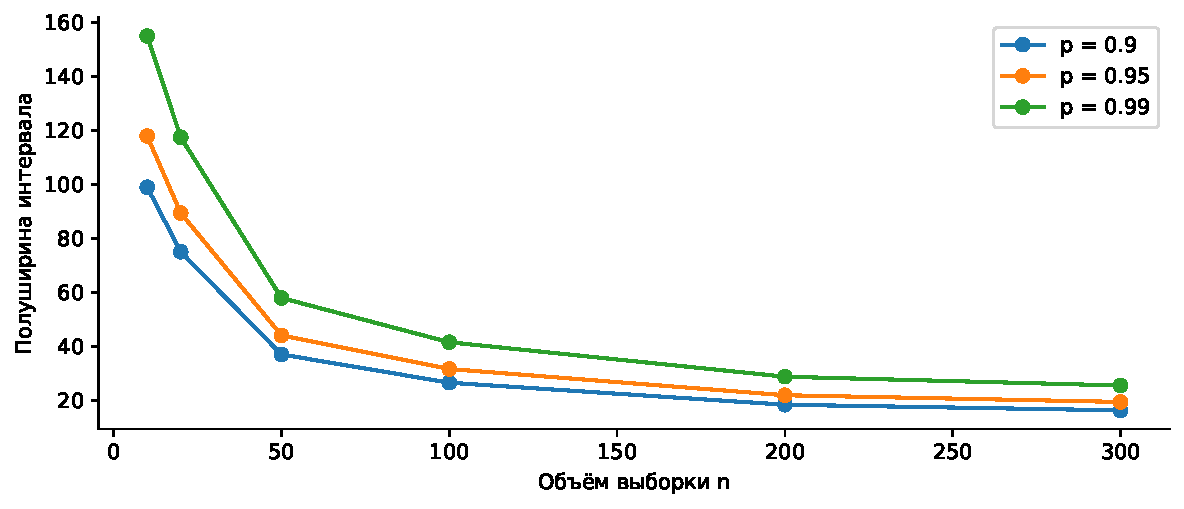
\includegraphics[width=.74\linewidth]{ci.pdf}\caption{Зависимость полуширины доверительного интервала от объёма выборки}
\end{figure}
При фиксированном $n$ более высокая доверительная вероятность требует более широкого интервала. При росте $n$ множитель $1/\sqrt n$ уменьшает его ширину, хотя одновременно меняется оценка $s_n$.

\section{Характер последовательности и гистограмма}
\begin{figure}[H]\centering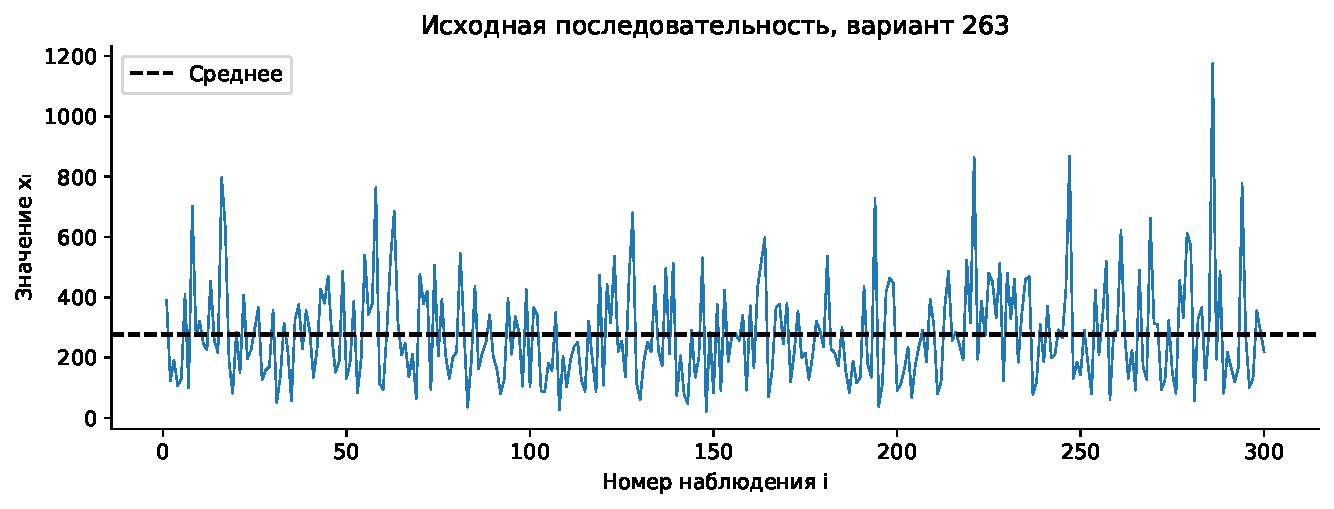
\includegraphics[width=\linewidth]{original.pdf}\caption{График 1. Значения исходной последовательности}
\end{figure}
На графике наблюдаются нерегулярные колебания с отдельными большими значениями. Последовательность не является монотонно возрастающей или убывающей. Повторяющийся период визуально не выделяется. В качестве дополнительной проверки оценён линейный тренд: наклон 0.109897 на один номер наблюдения, двустороннее $p$-значение 0.3364. На уровне 0.05 значимого линейного тренда не обнаружено. Этот результат сам по себе не доказывает стационарность.
\begin{figure}[H]\centering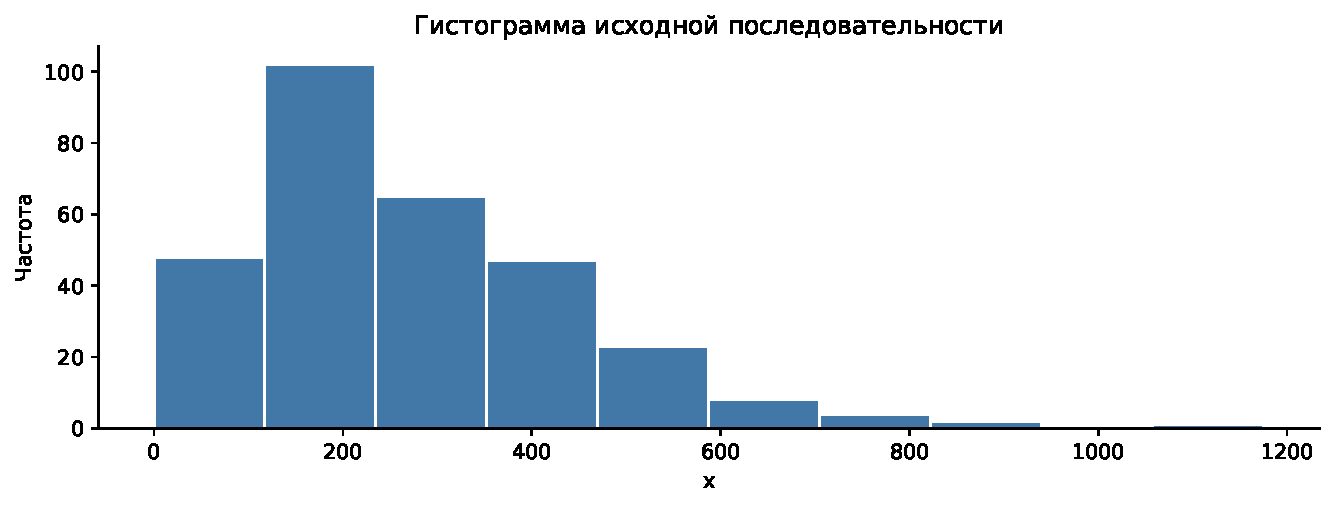
\includegraphics[width=\linewidth]{hist_original.pdf}\caption{График 2. Частоты исходной последовательности в 10 равных интервалах}
\end{figure}
Гистограмма показывает положительную асимметрию и правый хвост. Для сопоставления обеих выборок используются одинаковые 10 интервалов от нуля до общего максимума. Интервалы замкнуты слева и открыты справа, последний включает правую границу. Выбор числа интервалов влияет на внешний вид гистограммы, поэтому дополнительно рассматривается расстояние между эмпирической и теоретической функциями распределения.

\section{Автокорреляционный анализ}
Используем корреляцию Пирсона двух укороченных последовательностей $(x_1,\ldots,x_{N-k})$ и $(x_{1+k},\ldots,x_N)$:
\begin{equation}
r_x(k)=\frac{\sum_{i=1}^{N-k}(x_i-\bar x_L)(x_{i+k}-\bar x_R)}
{\sqrt{\sum_{i=1}^{N-k}(x_i-\bar x_L)^2\sum_{i=1}^{N-k}(x_{i+k}-\bar x_R)^2}}.
\end{equation}
Средние $\bar x_L,\bar x_R$ рассчитаны отдельно для соответствующих отрезков. В таблице приведены обязательные сдвиги 1--10, на графике --- 1--60. При больших сдвигах число пар уменьшается и оценка становится менее устойчивой.
\begin{table}[H]\centering\caption{Форма 3. Автокорреляция исходной и сгенерированной последовательностей}
\small\begin{tabular}{rrrrr}\toprule
$k$ & $r_x(k)$ & $r_y(k)$ & $\Delta r$ & $\Delta,\%$ \\\midrule
1 & -0.0327 & -0.0340 & -0.0013 & -3.90 \\
2 & -0.0317 & -0.0461 & -0.0144 & -45.34 \\
3 & -0.0440 & 0.0203 & 0.0643 & 146.16 \\
4 & -0.0031 & -0.1060 & -0.1029 & -3313.46 \\
5 & 0.0225 & -0.0921 & -0.1147 & -508.85 \\
6 & 0.0470 & 0.0053 & -0.0417 & -88.81 \\
7 & 0.0330 & -0.0029 & -0.0359 & -108.81 \\
8 & 0.0790 & 0.0310 & -0.0480 & -60.73 \\
9 & 0.0632 & -0.0755 & -0.1387 & -219.60 \\
10 & -0.0445 & 0.1123 & 0.1569 & 352.15 \\
\bottomrule\end{tabular}\end{table}
Здесь $\Delta r=r_y-r_x$, а $\Delta,\%=100(r_y-r_x)/|r_x|$. Процентные различия приведены согласно форме задания, но при $r_x\approx0$ они неустойчивы и не характеризуют качество модели. Например, малый знаменатель при $k=4$ даёт большое процентное отличие при умеренной абсолютной разности.
\begin{figure}[H]\centering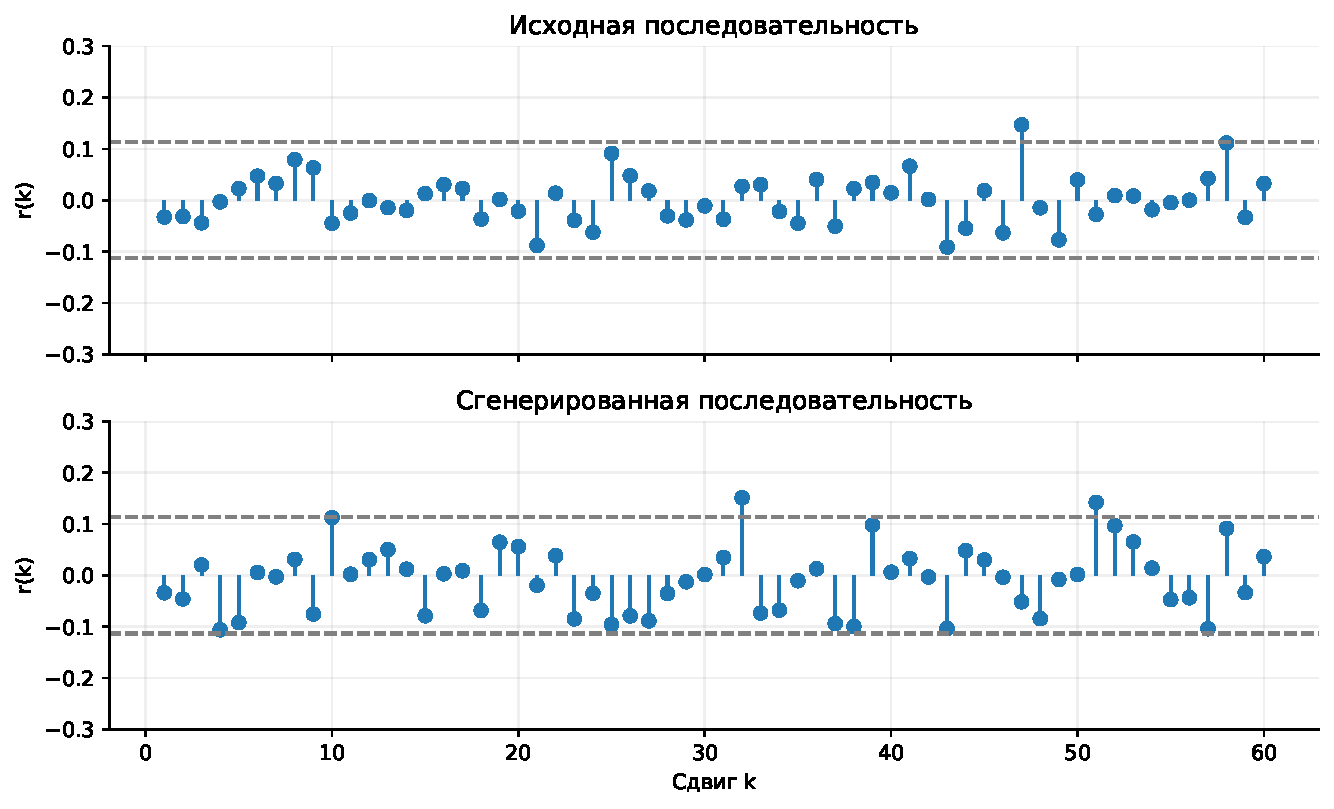
\includegraphics[width=.74\linewidth]{acf.pdf}\caption{Автокорреляционные функции. Пунктир: ориентировочные поточечные границы $\pm1.96/\sqrt{300}=\pm0.1132$}
\end{figure}
Границы являются диагностическим ориентиром для белого шума, а не одновременной гарантией для всех сдвигов. На сдвигах 1--10 все коэффициенты обеих последовательностей находятся внутри этих границ. Регулярной периодической структуры не выявлено. Нулевая линейная корреляция не доказывает независимость или случайность.

Дополнительно применён критерий Льюнга--Бокса для первых 10 сдвигов:
\begin{equation}
Q=N(N+2)\sum_{k=1}^{10}\frac{\widehat\rho_k^2}{N-k},\qquad
\widehat\rho_k=\frac{\sum_{i=1}^{N-k}(x_i-\bar x)(x_{i+k}-\bar x)}{\sum_{i=1}^N(x_i-\bar x)^2}.
\end{equation}
Для этого критерия используется стандартная нормировка с общим средним, отличающаяся от корреляции укороченных отрезков в форме 3. Для исходной последовательности $Q=5.8741$, $p=0.8257$; для сгенерированной $Q=12.5094$, $p=0.2524$. При уровне значимости 0.05 гипотеза отсутствия автокорреляции на первых 10 сдвигах не отвергается для обеих выборок. Совместно с графиками это позволяет использовать модель независимых случайных наблюдений в рамках работы, но не устанавливает механизм происхождения исходных данных.

\section{Аппроксимация по двум моментам}
Второй начальный выборочный момент равен
\[
\widehat m_{2,\mathrm{raw}}=\frac1{300}\sum x_i^2=105640.708853.
\]
Для согласования с несмещённой дисперсией из формы 1 используем оценки моментов $m_1=\bar x$ и $m_2=\bar x^2+s^2=105738.369429$. Их отличие от сырого момента равно $s^2/300=97.660577$. Тем самым закон согласован с оценённой дисперсией $s^2$, а не с дисперсией с делителем $N$.

Получено $v^2=0.3832823$, $1/v^2\approx2.6090$. Экспоненциальный закон требует $v=1$, гиперэкспоненциальный --- $v\geq1$. Равномерный закон, согласованный с этими моментами, имел бы левую границу $\bar x-\sqrt3s\approx-19.99$, то есть допускал бы отрицательные значения. У неотрицательного равномерного распределения $v\leq1/\sqrt3\approx0.5774$. Нормированный закон Эрланга порядка 3 имеет $v=1/\sqrt3$ и не воспроизводит найденную вариацию точно.

Выберем гипоэкспоненциальный закон: сумму трёх независимых экспоненциальных стадий с двумя одинаковыми средними:
\[
Y=E_1+E_2+E_3,\quad E_1,E_2\sim\operatorname{Exp}(1/a),\quad
E_3\sim\operatorname{Exp}(1/b).
\]
Условия согласования моментов: $2a+b=m_1$, $2a^2+b^2=s^2$. Выбранное решение
\begin{equation}
a=\frac{m_1-\sqrt{(3s^2-m_1^2)/2}}{3}=66.933397,\qquad
b=m_1-2a=142.611408.
\end{equation}
Оно положительно при $1/3\leq v^2<1$. Интенсивности равны $\lambda_a=0.0149402248$, $\lambda_b=0.0070120617$. Проверка даёт $E[Y]=276.478202$ и $D[Y]=29298.173051$. Два момента не определяют распределение однозначно: выбран простой положительный фазовый закон с минимальным необходимым числом экспоненциальных стадий, так как для суммы $k$ таких стадий $v^2\geq1/k$.

\section{Алгоритм генерации и характеристики новой выборки}
Плотность выбранного закона при $t\geq0$ имеет вид
\begin{equation}
f_Y(t)=\frac{\lambda_a^2\lambda_b}{(\lambda_a-\lambda_b)^2}
e^{-\lambda_b t}\left[1-e^{-(\lambda_a-\lambda_b)t}\bigl(1+(\lambda_a-\lambda_b)t\bigr)\right],
\end{equation}
а при $t<0$ равна нулю. Она получена свёрткой плотности Эрланга порядка 2 и экспоненциальной плотности. В программе график вычисляется через эквивалентное фазовое представление, чтобы избежать вычитания близких чисел при малом $t$.

Для каждого $i$ генерируются независимые равномерные числа $U_{i1},U_{i2},U_{i3}\in[0,1)$, после чего
\begin{equation}Y_i=-a\ln(1-U_{i1})-a\ln(1-U_{i2})-b\ln(1-U_{i3}).\end{equation}
Для трёх стадий применён генератор равномерных чисел с фиксированным начальным состоянием. Сформированы 300 значений без последующей подгонки или масштабирования. При другом начальном состоянии получится новая реализация того же закона. В форме 2 проценты рассчитаны относительно исходной выборки того же объёма.

\subsection{Программа обработки и контрольный запуск}
Программа последовательно считывает 300 измерений, определяет параметры $a$ и $b$, формирует новую последовательность методом обратной функции распределения и для первых $n=10,20,50,100,200,300$ элементов каждой последовательности вычисляет $\bar x_n$, $s_n^2$, $s_n$, $v_n$ и полуширины трёх доверительных интервалов. Затем она рассчитывает автокорреляцию при сдвигах 1--10, частоты в десяти общих интервалах и коэффициент корреляции исходной и сгенерированной последовательностей. Полный исполняемый пример приведён в листинге 1.

\begin{center}\textbf{Листинг 1. Генерация и расчёт числовых характеристик}\end{center}
\VerbatimInput[fontsize=\scriptsize,numbers=left,numbersep=5pt]{code/report_demo.py}

Контрольный запуск дал $a=66.933397$, $b=142.611408$. Первые пять сгенерированных значений: $47.212$, $110.139$, $412.266$, $84.040$, $495.475$. Для полной выборки программа получила $\bar y=262.501$, $s_y^2=25732.224$, $s_y=160.413$, $v_y=0.6111$ и полуширины $15.234$, $18.152$, $23.856$ при вероятностях $0.90$, $0.95$, $0.99$. Обе гистограммы содержат по 300 наблюдений. Результаты совпадают с формой 2 после округления; при демонстрации можно изменить начальное состояние генератора и убедиться, что значения меняются, сохраняя закон распределения.
\begin{table}[H]\centering\caption{Форма 2. Характеристики гипоэкспоненциальной последовательности}
\small\setlength{\tabcolsep}{4pt}\begin{tabular}{lrrrrrr}\toprule
Показатель & 10 & 20 & 50 & 100 & 200 & 300 \\\midrule
$\bar x$ & 248.3056 & 289.2477 & 276.1503 & 269.4767 & 269.7020 & 262.5007 \\
$\Delta,\%$ & -9.38 & -5.46 & 0.09 & -2.70 & 1.74 & -5.06 \\\addlinespace
$s^2$ & 34556.9062 & 35083.7747 & 33677.3883 & 29839.0038 & 25892.0977 & 25732.2238 \\
$\Delta,\%$ & -4.55 & -15.66 & 33.28 & 14.95 & 4.10 & -12.17 \\\addlinespace
$s$ & 185.8949 & 187.3066 & 183.5140 & 172.7397 & 160.9102 & 160.4127 \\
$\Delta,\%$ & -2.30 & -8.16 & 15.45 & 7.22 & 2.03 & -6.28 \\\addlinespace
$v$ & 0.7487 & 0.6476 & 0.6645 & 0.6410 & 0.5966 & 0.6111 \\
$\Delta,\%$ & 7.81 & -2.86 & 15.34 & 10.19 & 0.28 & -1.29 \\\addlinespace
$\varepsilon_{0.90}$ &  $\pm 96.6929$ &  $\pm 68.8915$ &  $\pm 42.6886$ &  $\pm 28.4132$ &  $\pm 18.7153$ &  $\pm 15.2337$ \\
$\Delta,\%$ & -2.30 & -8.16 & 15.45 & 7.22 & 2.03 & -6.28 \\\addlinespace
$\varepsilon_{0.95}$ &  $\pm 115.2167$ &  $\pm 82.0892$ &  $\pm 50.8666$ &  $\pm 33.8564$ &  $\pm 22.3006$ &  $\pm 18.1521$ \\
$\Delta,\%$ & -2.30 & -8.16 & 15.45 & 7.22 & 2.03 & -6.28 \\\addlinespace
$\varepsilon_{0.99}$ &  $\pm 151.4204$ &  $\pm 107.8836$ &  $\pm 66.8500$ &  $\pm 44.4948$ &  $\pm 29.3080$ &  $\pm 23.8559$ \\
$\Delta,\%$ & -2.30 & -8.16 & 15.45 & 7.22 & 2.03 & -6.28 \\\addlinespace
\bottomrule\end{tabular}\end{table}
При $n=300$ среднее новой выборки равно 262.500701 (отклонение $-5.0556\%$), дисперсия 25732.223755 ($-12.1712\%$), стандартное отклонение 160.412667 ($-6.2830\%$), коэффициент вариации 0.611094 ($-1.2928\%$). Совпадение теоретических моментов не означает их точного совпадения в конечной случайной реализации. Среднее генератора находится внутри исходного приближённого 95\%-интервала; это описательное сравнение, а не самостоятельный критерий равенства распределений.

\section{Сопоставление последовательностей и распределений}
\begin{figure}[H]\centering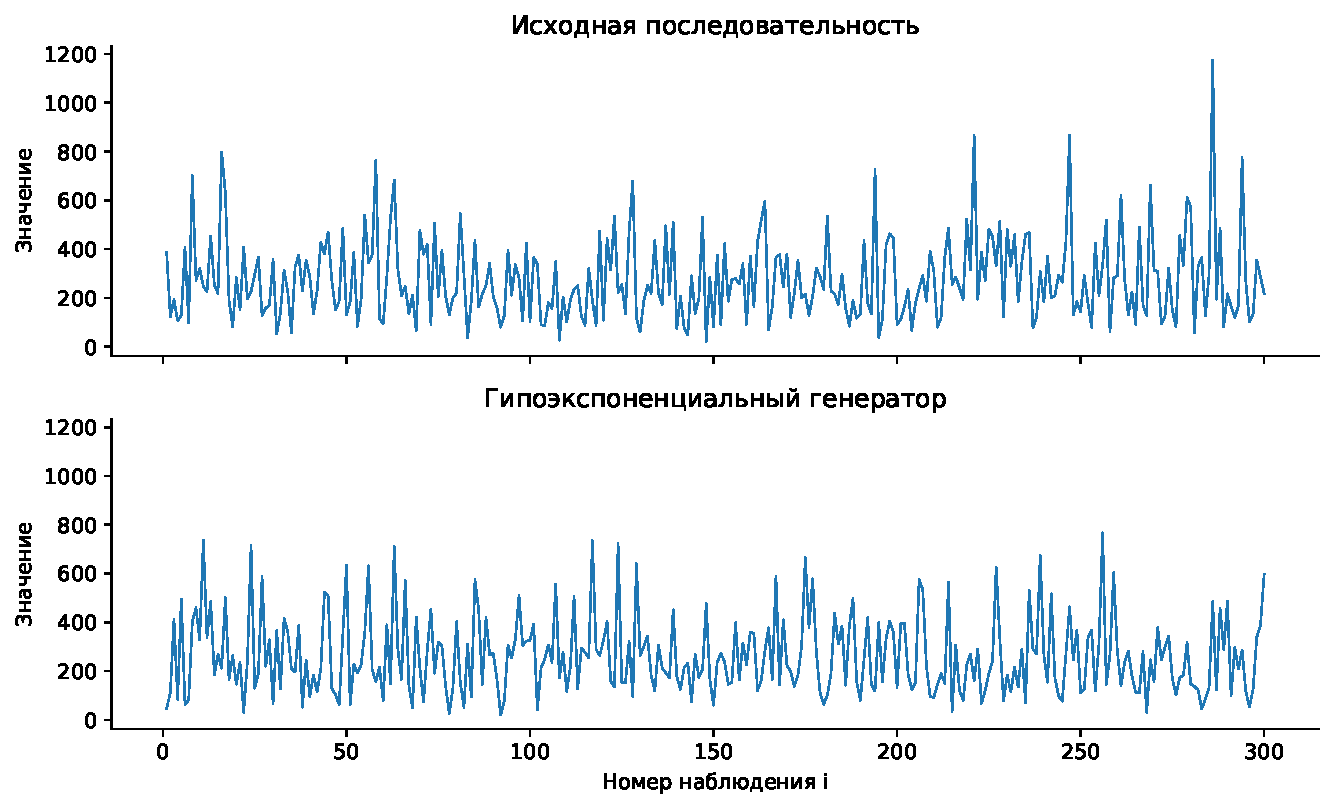
\includegraphics[width=.96\linewidth]{comparison.pdf}\caption{Сравнение значений исходной и сгенерированной последовательностей}
\end{figure}
Сопоставимые масштабы и отдельные большие значения воспроизводятся. Совпадение значений при одинаковом номере наблюдения не ожидается: генератор моделирует закон распределения, а не повторяет исходную траекторию.
\begin{figure}[H]\centering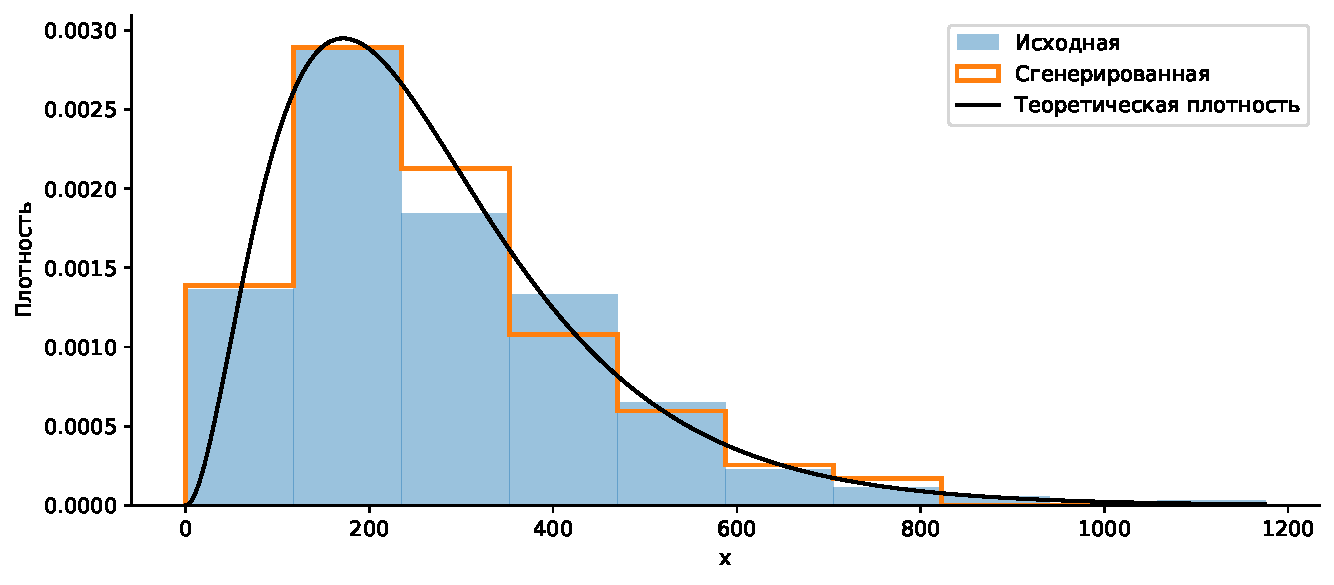
\includegraphics[width=.96\linewidth]{density.pdf}\caption{График 3. Теоретическая плотность и нормированные гистограммы обеих выборок}
\end{figure}
Высота столбца нормированной гистограммы равна $n_j/(Nh)$, поэтому её площадь равна единице и она сопоставима с плотностью. Модель воспроизводит основную массу наблюдений и правую асимметрию. Расхождения в отдельных интервалах ожидаемы при 300 наблюдениях; крайние интервалы содержат мало значений, поэтому качество описания хвоста оценивается менее уверенно.

\begin{table}[H]\centering\caption{Частоты на общих интервалах и ожидаемые частоты модели}
\small\begin{tabular}{rrrrr}\toprule
Левая граница & Правая граница & $n_x$ & $n_y$ & $300p_j$ \\\midrule
0.00 & 117.53 & 48 & 49 & 45.41 \\
117.53 & 235.05 & 102 & 102 & 100.27 \\
235.05 & 352.58 & 65 & 75 & 75.56 \\
352.58 & 470.10 & 47 & 38 & 41.66 \\
470.10 & 587.63 & 23 & 21 & 20.27 \\
587.63 & 705.15 & 8 & 9 & 9.33 \\
705.15 & 822.68 & 4 & 6 & 4.18 \\
822.68 & 940.21 & 2 & 0 & 1.85 \\
940.21 & 1057.73 & 0 & 0 & 0.82 \\
1057.73 & 1175.26 & 1 & 0 & 0.36 \\
\bottomrule\end{tabular}\end{table}
Теоретическая вероятность интервала вычисляется как $p_j=F(b_j)-F(a_j)$. Модель не обрезана на максимуме выборки: за последней границей остаётся положительная теоретическая вероятность, поэтому сумма ожидаемых частот в таблице несколько меньше 300.

Максимальное расстояние $D=\sup_t|F_{300}(t)-F_Y(t)|=0.042858$ характеризует различие эмпирической и подобранной функций распределения. Оно приведено как описательная мера. Обычное $p$-значение критерия Колмогорова для полностью заданного распределения здесь неприменимо, поскольку параметры оценены по той же выборке. Расстояние между двумя эмпирическими функциями распределения равно 0.073333.

\subsection{Корреляция между исходной и новой последовательностями}
Коэффициент Пирсона для пар $(x_i,y_i)$ равен
\[
r_{xy}=\frac{\sum_{i=1}^{300}(x_i-\bar x)(y_i-\bar y)}{\sqrt{\sum(x_i-\bar x)^2\sum(y_i-\bar y)^2}}=0.074452.
\]
Это слабая линейная связь. Приближённое двустороннее $p$-значение стандартного теста Пирсона равно 0.1985: значимой линейной связи на уровне 0.05 не обнаружено. Параметры генератора оценены по исходным данным, поэтому полную статистическую независимость результатов всего процесса подбора утверждать нельзя. Однако при зафиксированных параметрах новые случайные числа формируются отдельно от исходных значений.

\section{Заключение}
Для исходной выборки объёмом 300 наблюдений получены $\bar x=276.4782$, $s^2=29298.1731$ и $v=0.6191$. Интервал для среднего расширяется с ростом доверительной вероятности. Монотонности и устойчивой периодичности не выявлено; автокорреляция на первых десяти сдвигах не противоречит модели некоррелированных наблюдений. По двум моментам выбран трёхстадийный гипоэкспоненциальный закон. Генератор воспроизводит положительную асимметрию и масштаб разброса: отклонения среднего и дисперсии новой выборки составили $-5.06\%$ и $-12.17\%$. Точность описания редкого правого хвоста по 300 наблюдениям ограничена.
\end{document}


